
%%
%%  This file was updated in April 2009 by J. Poole to be in line with Word tempaltes
%%
%%  Use \documentclass[boxit]{jacow}
%%  to draw a frame with the correct margins on the output.
%%
\documentclass{jacow}
%\documentclass{article}
%\usepackage{mathtools}
\usepackage{amsmath}
%%  for US letter paper layout
%%
\usepackage{graphicx}
\usepackage{booktabs}
%%
%%   VARIABLE HEIGHT FOR THE TITLE BOX (default 35mm)
%%

\setlength{\titleblockheight}{27mm}

\begin{document}
\title{The Development of Stochastic Processes in COSY Infinity}

\author{J. Kunz\thanks{jkunz@hawk.iit.edu}, P. Snopok, Illinois Institute of Technology, Chicago, IL 60616, USA\\
        M. Berz, K. Makino, Michigan State University, East Lansing, MI 48824, USA}

\maketitle

\begin{abstract}
COSY Infinity is an arbitrary-order beam dynamics simulation and analysis code. It can determine high-order transfer maps of combinations of particle optical elements of arbitrary field configurations. For precision modeling, design, and optimization of next-generation muon beam facilities, its features make it a very attractive code. Certain new features are being developed for inclusion in COSY to follow the distribution of charged particles through matter. To study in detail some of the properties of muons passing through material, the transfer map approach alone is not sufficient. The interplay of beam optics and atomic processes must be studied by a hybrid transfer map--Monte-Carlo approach in which transfer map methods describe the average behavior of the particles in the accelerator channel including energy loss, and Monte Carlo methods are used to provide small corrections to the predictions of the transfer map accounting for the stochastic nature of scattering and straggling of particles. The advantage of the new approach is that it is very efficient in that the vast majority of the dynamics is represented by fast application of the high order transfer map of an entire element and accumulated stochastic effects as well as possible particle decay. The gains in speed are expected to simplify the optimization of muon cooling channels which are usually very computationally demanding due to the need to repeatedly run large numbers of particles through large numbers of configurations. Progress on the development of the required algorithms is reported.
\end{abstract}

\section{INTRODUCTION}
COSY Infinity is a beamline simulations tool used in the design, analysis, and optomization of particle accelerators [1]. To do this, COSY uses the transfer map approach, which evaluates the overall effect of a system on a beam of particles  using differential algebra (involving multivariate Taylor polynomials up to arbitrary order). While a transfer map is technically not a nonlinear matrix, it is sometimes helpful to think of them as one in the same. Along with the evaluation of particles through a lattice, COSY also has a plethora of analysis and optomization tools, including (but not limited to) lattice aberration and correction tools, support for Twiss parameters, support for tunes and nonlinear tune shifts, built-in optimizers (for lattice design), and spin tracking. \par

COSY is particularly advantageous to use when considering the efficient use of computational time. This is due to the transfer map methods that COSY employs. Given some initial phase space vector
\begin{equation}
\mathbf{Z}=
\begin{pmatrix}
x\\ y\\ l=k(t-t_0)\\a=p_x/p_0\\b=p_y/p_0\\  \delta = (E-E_0)/E_0
\end{pmatrix}
\end{equation}
where the so-called particle optical coordinates are transverse positions ($x, y$), time-of-flight in units of length ($l$), transverse angles w.r.t. the reference particle ($a, b$), and kinetic energy deviations w.r.t. the reference particle ($\delta$), and the $0$ subscript in the definitions denotes the reference particle's properties, the transfer map $\mathcal{M}$ will uniquely predict the time evolution of $\mathbf{Z}$. This is because most beam elements follow Maxwell's equations, which yield unique solutions that are dependent on initial conditions. Mathematically, this relationship is $\mathbf{Z}(s)=\mathcal{M}(s_0 , s)*\mathbf{Z}(s_0)$. Here, the independent variable $s$ is understood as the reference orbit (the zero point of a beam of particles in some comoving reference frame --see Figure 2). Now, the composition of two maps yeilds another map: $\mathcal{M}(s_1 , s_2)\times \mathcal{M}(s_0 , s_1) = \mathcal{M}(s_0 , s_2)$. Therefore, it is possible to "cut out" the middle part $s_1$. Since each physical lattice corresponds to some transfer map, it is possible to construct a single map that represents many individual lattices. Computationally this is advantageous because once calculated, it is much faster to apply a solitary transfer map to a distribution of particles than to simulate that same distribution through many meters of lattices.
\par


Currently supported elements in COSY include but are not limited to: various magnetic and electric multipoles (with fringing effects), homogeneous and inhomogeneous bending elements, Wien filters, wigglers and undulators, cavities, cylindrical electromagnetic lenses, general particle optical elements, and deterministic polynomial absorbers of arbitrary order, with the last element being of particular interest. \par

\begin{figure}[h!]
\centering
\includegraphics*[width=70mm]{C:/Users/kunzj_000/Desktop/dissertation_mats/figure2}
\caption{The reference orbit.}
\end{figure}

The term $deterministic$ is deliberately emphasized, since the polynomial absorber acts like a simple drift with Bethe-Bloch energy loss. The advantage of this is that the user must only specify 6 material parameters in order for COSY to calculate this energy loss; in particular, the user must specify the Z number, A number, density, ionization potential, density correction parameter, and shell correction parameter. \par

However, this element only takes into account deterministic effects (effects which produce the same final result every time for some initial condition), not stochastic effects (pseudorandom effects such as multiple scattering and straggling). For a realistic simulation of a beam of particles through matter, one needs to take into account both the former and the latter. Eq.~\eqref{emittance} describes the normalized transverse emittance, where $\epsilon_n$ is the normalized emittance, $z$ is the path length, $E_\mu$ is the muon beam energy, $\beta = v/c$, $L_R$ is the radiation length of the absorber material, $\beta_\perp$ is the betatron function, and $E_s$ is the characteristic scattering energy [3,4].

\begin{equation}
\frac{d\epsilon_n }{dz} \approx -\frac{1}{\beta^2} \left< \frac{dE_\mu}{dz} \right> \frac{\epsilon_n}{E_\mu} + \frac{1}{\beta^3} \frac{\beta_\perp E_s ^2}{2E_\mu mc^2 L_R}
\label{emittance}
\end{equation}

Here, two competing effects can be seen: the first term is the cooling (reduction of phase space) component from ionization energy loss and the second term is the heating (enlargement of phase space) term from multiple scattering. This highlights the importance of the stochastic terms, as the only deterministic term is the expected (Bethe-Bloch) energy loss, $\left< \frac{dE_\mu}{dz} \right>$. \par

It is clear why stochastic effects do not fit well into the transfer map paradigm. To illustrate this, suppose that there are two identical particles with identical initial coordinates. As seen in Figure 3, one particle may scatter upwards and follow the yellow path and the other (due to the random nature of multiple scattering) may just happen to scatter downwards and follow the black path. Therefore, it is not possible to construct a traditional transfer map that represents the absorber. This would require uniquely relating the coordinates after the absorber to the coordinates before the absorber. \par

\begin{figure}[h!]
\centering
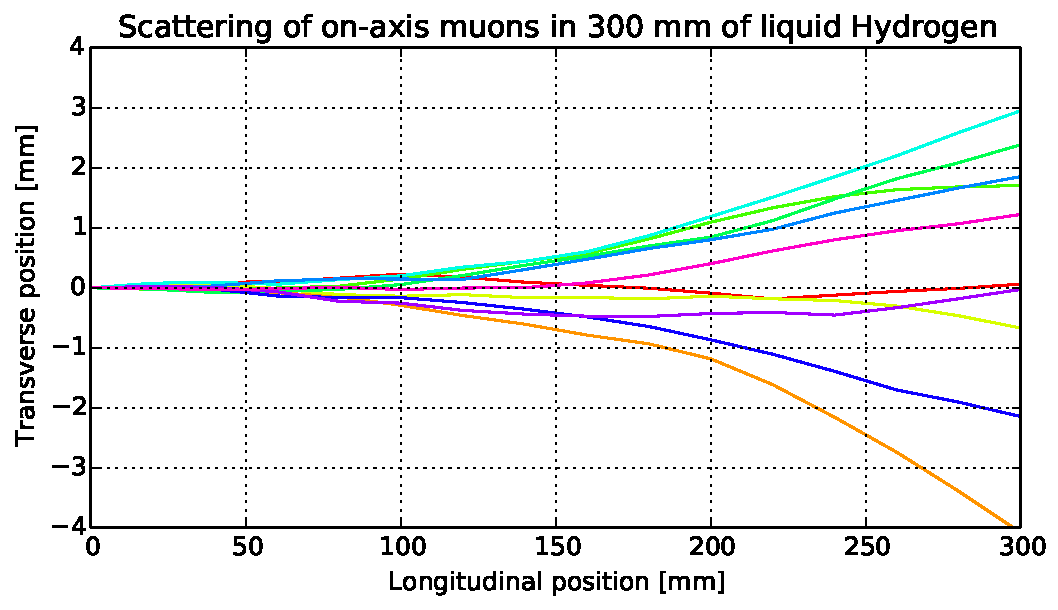
\includegraphics[width=0.49\textwidth]{figures/p10tr.pdf}
\caption{Possible scatterings of a particle through matter. Due to the random nature of multiple scattering, a particle may scatter at a variety of angles when traversing matter.}
\end{figure}

To further stress the importance of stochastic effects as a part of realistic simulations, COSY was compared to another program called ICOOL [2]. This was done by the simulation of a flat 32 cm liquid hydrogen absorber proceeded and followed by 10 cm drifts. ICOOL is a particle-by-particle propagation code written for the study of ionization cooling of muon beams. Therefore, the discrepancy between these two codes is largely due to stochastic effects. The results of this simulation are found in Table 1. Here, it is clear that while the longitudinal coordinates appear to agree well, the transverse coordinates do not. Moreover, the large discrepancy between the X and Y percent disagreements is likely because the initial distributions were randomly centered about (X, Px, Y, Py) = (0, 0, 0, 0).

\begin{table}[hbt]
   \centering
   \caption{Results of a comparison simulation between COSY and ICOOL. The simulation was of a 32 cm flat liquid hydrogen absorber proceeded and followed by 10 cm drifts. The discrepancy between the two codes is understood as whether or not the code consideres stochastic effects.}
   \begin{tabular}{lcccc}
       \toprule
			 \textbf{}            & \textbf{Initial} 	& \textbf{Final (COSY)} & \textbf{Final (ICOOL)} 	& \textbf{\% Disagreement (w.r.t. ICOOL)} \\ 
          $ X (mm)$      &0.001572 &-1.862 &-1.756 &6.04\\
	$\sigma_X (mm)$&0.967&26.617&27.150&1.96\\
	$P_X (MeV)$&-3.584&-0.6612&-0.6120&8.04\\
	$\sigma_{P_X} (MeV)$&51.151&9.498&9.899&4.05\\
	$Y (mm)$&0.018172&-0.8227&-1.055&22.02\\
	$\sigma_Y (mm)$&1.035&26.080&26.050&0.12\\
	$P_Y (MeV)$&-1.617&-.373&-0.4490&31.56\\
	$\sigma_{P_Y} (MeV)$&50.234&9.331&9.423&0.98\\
	$P (MeV)$&200.228&189.173&189.114&0.03\\
	$\sigma_P (MeV)$&19.883&20.534&20.528&0.03\\
       \bottomrule
   \end{tabular}
   \label{l2ea4-t1}
\end{table}

However, here it is important to note that the standard deviation of the longitudinal coordinates may not be well-defined, as the energy loss of particles through a material follows a Landau distribution, not Gaussian. This was not accounted for until recently, and as such the standard deviation was used in spite of this fact. \par

\section{MOTIVATION}

A prime example of why matter-dominated lattices are relevant comes from the prospect of a muon accelerator. While the Large Hadron Collider is roughly 27 km in circumference and the next proposed hadron collider could be up to 50 km, a high energy muon collider ($\sqrt{s}=$ 6.0 TeV) could be built on the existing Fermilab site (roughly 6 km in circumference) [8]. Additionally, a muon collider could serve as a Higgs factory ($\sqrt{s}=$126 GeV), with possible new physics via the observation of Higgs to lepton coupling. Moreover, as muon branching fractions are 100\% neutrino-antineutrino, there are obvious advantages of a muon-sourced neutrino beam. \par

However, muon-based facilities are not without their challenges. Muons are unstable particles, and have a rest-frame lifetime of 2.2 $\mu$s. Therefore, beam cooling techniques which are used for protons and electrons cannot be used, as they are too slow. Synthetic muon creation comes from the collision of protons on a fixed target. The resultant spray of particles largely contains kaons (which decay primarily into pions and muons), pions (which decay primarily into muons), and rogue protons. Therefore, high-intensity collection necessitates a large initial phase space volume. The resultant cloud of muons must be collected, focused, and accelerated well within the muon lifetime (2.2 $\mu$s). Due to the short-lived nature of the muon, novel beam cooling (beam size reduction) techniques have been explored and 6D ionization cooling in particular has been shown to work quite well [5,6]. Muons traverse a certain amount of material in order to lose energy in both longitudinal and transverse direction due to ionization. The energy is then manually restored in the longitudinal direction only, leading to an overall reduction in the transverse direction (cooling). In order to achieve cooling in the longitudinal direction, emittance exchange is used, usually involving wedge-shaped absorbers. The result of such an emittance exchange scheme can be seen in Figure 4 [7]. \par

\begin{figure}[h!]
\centering
\includegraphics*[width=70mm]{C:/Users/kunzj_000/Desktop/dissertation_mats/figure4}
\caption{Emittance exchange.}
\end{figure}


\section{STOCHASTIC PROCESSES IN COSY AND PRELIMINARY RESULTS}
It has been shown that the inclusion of stochastic processes into COSY Infinity would be both necessary for realistic simulation and relevant to future experiments. Towards this end, new subroutines have been entered into COSY which would accurately take into account stochastic effects without compromising COSY's computational efficiency when compared to similar codes. These subroutines are designed to apply a perturbative kick to each particle at the end of the absorber, thereby emulating stochastic effects. The strength and variety of this kick depends on two parameters: the initial energy of the particle and the length of absorber that the particle traverses (equivalently, the average amount of energy lost within the material). This can be done because the particle's coordinates follow predictable paterns when it travels through matter, as can be seen by Figures 5 and 6 (raw data generated by ICOOL [2], another program which takes into account stochastic effects). \par

\begin{figure}[h!]
\centering
\includegraphics*[width=80mm]{C:/Users/kunzj_000/Desktop/dissertation_mats/figure5}
\caption{Transverse position histograms for four different absorber lengths corresponding to 5, 10, 15, and 20 MeV/c momentum loss. The initial distribution was a pencil beam of 10,000 muons with an initial momentum of 200 MeV/c. The histograms follow a Gaussian curve.}
\end{figure}

\begin{figure}[h!]
\centering
\includegraphics*[width=80mm]{C:/Users/kunzj_000/Desktop/dissertation_mats/figure6}
\caption{Energy loss histograms for four different absorber lengths corresponding to 5, 10, 15, and 20 MeV/c momentum loss. The initial distribution was a pencil beam of 10,000 muons with an initial momentum of 200 MeV/c. The histograms follow a Landau curve.}
\end{figure}

When COSY applies the effects of an absorber onto a distribution of particles, two events occur: the transfer map method of the application of deterministic effects and the new method of applying a random kick to each particle's coordinates. To exemplify this, observe from Figure 5 that the transverse position of a particle follows a Gaussian curve. The mean parameter $\mu$ of this curve is always zero (i.e. the particle effectively goes in a straight line on average). The standard deviation parameter $\sigma$, however, clearly varies depending on the pathlength through the absorber, which COSY conveniently already calculates as part of the transfer map method. Therefore, it is possible to represent the $\sigma$ parameter as a function of initial energy and absorber length. For this reason, this method and its collective subroutines have been referred to as the "functional method". Figure 7 shows an example plot of $\sigma$ versus average energy loss (equivalently, absorber length) for a pencil beam of 10,000 muons with an initial momentum of 200 MeV/c. The various colors represent the initial random seed. The function $\sigma (\Delta E)$ can be obtained by averaging similar $\sigma$s and curve fitting these results parabolically. \par

\begin{figure}[h!]
\centering
\includegraphics*[width=80mm]{C:/Users/kunzj_000/Desktop/dissertation_mats/figure7}
\caption{$\sigma$ versus average $\Delta$E.}
\end{figure}

To test this method, an on-center Gaussian distribution of 10,000 muons with parameters ($\sigma_X, \sigma_{P_X}$) = ($10 mm, 10 keV$) and initial momenta of 200 MeV/c ($\sigma_{P_Z} = 0$) was generated and simulated through a 32 cm liquid hydrogen absorber. The absorber geometry was triangular prismatic with 45 degree opening and closing angles and was proceeded and followed by 10 cm drifts. This ensured that each particle went through a different absorber length. These conditions were simulated in COSY without the functional method, COSY with the functional method, and three different ICOOL [2] runs where the random seed was changed. The results can be seen in Table 2.

\begin{table}[hbt]
   \centering
   \caption{COSY vs Functional COSY vs ICOOL.}
   \begin{tabular}{lcccccc}
       \toprule
	\textbf{}& \textbf{COSY} & \textbf{Functional COSY}&\textbf{ICOOL 1}&\textbf{ICOOL 2}&\textbf{ICOOL 3}& \textbf{Average ICOOL} \\ 
          $ \sigma_X (mm)$&18.96&19.05&19.06&19.04&19.02&19.04\\
	$\sigma_Y (mm)$&19.00&19.06&19.17&19.10&19.10&19.12\\
	\bottomrule
   \end{tabular}
   \label{l2ea4-t1}
\end{table}

\section{FUTURE DIRECTIONS}
While Table 2 shows optomistic results for the functional method, the current development is quite preliminary. Some future work to be done includes:
\begin{itemize}
\item More testing (necessary due to the random nature of the functional method)
\item The correlation of parameters (e.g. the coupling between $\sigma_X$ and $\sigma_{P_X}$) 
\item Inclusion of the longitudinal coordinates
\item Comparison with other codes and experimental data
\item Functionalization which includes the initial energy as a parameter in addition to the absorber length
\item Funtionalization of different materials (only liquid hydrogen has been shown here)
\item Support for decay
\item Support for various particles or mixed beams
\item Absorbers inside of fields
\item Pressurized RF cavities
\end{itemize}
To this end, steady progress is being made, and it is anticipated that COSY will make use of the functional method for the efficient and robust simulation of particles through matter.

\begin{thebibliography}{9}   % Use for  1-9  references
%\begin{thebibliography}{99} % Use for 10-99 references

%\bibitem{a-ref} 
%COSY Infinity, \texttt{http://www.bt.pa.msu.edu}.
%[2] ICOOL, 2013, https://pubweb.bnl.gov/~fernow/icool/readme.html.


%\bibitem{a-ref} A. Example, \texttt{http://bt.pa.msu.edu/index_cosy.htm}.

\bibitem{COSY-ref} 
COSY Infinity, \texttt{http://www.bt.pa.msu.edu/index\_cosy.htm}
\bibitem{ICOOL-ref} 
ICOOL, \texttt{ https://pubweb.bnl.gov/~fernow/icool/readme.html}
\bibitem{Kim-ref}
E.S. Kim, M. Yoon, Design of Transverse Muon-Cooling Channels for a Neutrino Factory, Japan Journal of Applied Physics Vol. 40, pp. 401-406, 2001, \texttt{http://www-mucool.fnal.gov/mcnotes/public/pdf/muc0225/muc0225.pdf}.
\bibitem{Bravar-ref}
U. Bravar et al., MICE: the Muon Ionization Cooling Experiment, Proceedings of the DPF-2011 Conference, 2011, \texttt{http://arxiv.org/ftp/arxiv/papers/1110/1110.1813.pdf}.
\bibitem{MuScat-ref}
MuScat Collaboration, The scattering of muons in  low Z materials, 2005, \texttt{http://arxiv.org/abs/hep-ex/0512005}.
\bibitem{Fermilab-ref}
Fermilab, A Feasibility Study of a Neutrino Source Based on a Muon Storage Ring, edited by N. Holtkamp and D. Finley, 2000.
\bibitem{Palmer-ref}
M. Palmer, The R\&D Program For A Future Muon Collider, 2013, \texttt{http://accelconf.web.cern.ch/AccelConf/pac2013/talks/moyaa2\_talk.pdf}.
\bibitem{Eichten-ref}
E. Eichten, Physics at a Muon Collider Higgs Factory, 2013, \texttt{https://hepconf.physics.ucla.edu/higgs2013/talks/eichten.pdf}.



\end{thebibliography}
\end{document}
